% !TeX root = RJwrapper.tex
\title{dapper: Data Augmentation for Private Posterior Estimation in R}


\author{by Kevin Eng, Jordan A. Awan, Ruobin Gong, Nianqiao Phyllis Ju, and Vinayak A. Rao}

\maketitle

\abstract{%
This paper serves as a reference and introduction on using the dapper R package. It is an MCMC sampling framework which targets the exact posterior distribution given privitized data. The goal of this package is to provide researchers a tool for exploring the impact of different privacy regimes on a Bayesian analysis. A strength of this framework is the ability to target the exact posterior in settings where the likelihood is too complex to analytically express.
}

\hypertarget{introduction}{%
\section{Introduction}\label{introduction}}

Differential privacy provides a rigorous framework for protecting
confidential information (Dwork et al. 2006). It has served as the theoretical foundation for recent advances in privacy technology. Several high profile
examples include Apple (Tang et al. 2017), Google (Erlingsson, Pihur, and Korolova 2014), Microsoft (Ding, Kulkarni, and Yekhanin 2017), and the
U.S. Census Bureau (Abowd 2018).

Differential privacy works by injecting a suitable amount of
noise into a data analysis workflow and there are several approaches for modifying an existing workflow
to provide differentially private guarantees. These approaches mainly differ in where in the workflow privacy noise is injected.
Broadly speaking, noise can either be injected directly into a statistical estimating
procedure or into the data itself. (Ji, Lipton, and Elkan 2014)
provide a nice survey of how to modify several common machine learning algorithms
to be differentially private. The main drawback of this approach
is that it is model specific, so one needs to know before hand
what type of analysis is to be run.

In the case where noise is directly injected into the data, one can
consider the \emph{query} or \emph{dissemination} scenario (Hotz et al. 2022). In the query setting,
the user is only allowed to make specific request for summary statistics.
In the dissemination setting, full individual level micro data is released.
In both cases, privacy is maintained by adding noise directly to the released data product.
There is strong interest in further developing the query and dissemination approaches because data curators are often interested
in releasing data to the public without knowledge of how their data will
be used or analyzed. For a recent example of a high profile application of the dissemination approach
see the the U.S. Census Bureau's \texttt{TopDown} algorithm (Bureau 2023).

Correctly carrying out statistical inference in the dissemination setting
requires adjusting statistical workflows to account for privacy noise.
As an example, one instance of implementing the dissemination approach for tabular data involves directly
adding independent, random error to each cell. For regression models,
this corresponds to having data with measurement errors
in the covariates. This, unfortunately, violates the assumptions of most statistical models.
In the presence of such errors, standard estimators can exhibit significant bias and incorrect uncertainty quantification
(Gong 2022) (Karwa, Kifer, and Slavković 2015a) (Wang et al. 2018).
These issues are a serious concern for researchers (Santos-Lozada, Howard, and Verdery 2020) (Kenny et al. 2021) (Winkler et al. 2021).
Therefore, developing privacy aware statistical workflows is necessary in order
for science and privacy to coexists.

Unfortunately, making the necessary adjustments poses formidable mathematical
challenges (Williams and Mcsherry 2010), even for seemingly simple models like linear regression.
The difficulty can be seen from considering the marginal likelihood that results from correctly accounting for the injected
privacy noise. This function is often analytically intractable and as a result,
it is difficult or impossible to apply common maximum likelihood methods
to derive estimators. In particular, the marginal likelihood can involve a complex
integral where it is not possible to even evaluate the likelihood
at a point. This makes gradient based methods, like the Newton-Raphson method,
impractical. And approximating the likelihood can be computationally
unfeasible since the integral is also of high dimension.
Few tools are available to researchers to address these issues,
and their absence is a serious barrier to the wider adoption
of dissemination methods.

The \texttt{dapper} package provides a tool for conducting
valid statistical inference in the presence of privacy noise.
It implements the Bayesian framework proposed in (Ju et al. 2022). This framework describes how to modify
an existing Bayesian model to account for privacy noise. \texttt{dapper}
serves as user-friendly interface for implementing the framework in R. It allows the
user to specify a sampler from an existing Bayesian model and
automatically constructing a valid posterior sampler that accounts for the
added privacy noise. Compared to other Bayesian approaches, the \texttt{dapper} framework requires
no specialized knowledge for tuning samplers since there is no tuning parameter,
and when the record additivity is satisfied (see section 6), the algorithmic run time
complexity is similar to the non-private analysis. The goal of \texttt{dapper} is to provide
a fast, flexible, and user-friendly way to analyze the impact of privacy mechanisms.

The rest of this article is organized as follows. Section 2 covers the necessary background to understand the mathematical notation
and ideas used throughout the paper. Section 3 goes over the main algorithm without
going into mathematical detail, for specifics see (Ju et al. 2022). Section 4 provides
an overview of the dapper package and discusses important implementation details.
Section 5 contains two example of how one might use the package to analyze the
impact of adding noise for privacy. The first example goes over a typical
odds ratio analysis for a \(2 \times 2\) table and the second example
covers a linear regression model.

\hypertarget{background}{%
\section{Background}\label{background}}

Let \(x = (x_1, \ldots, x_n) \in \mathcal{X}^n\) represent a confidential
database containing \(n\) records. Usually, the goal of collecting data
is to learn some characteristic about the underlying population.
To accomplish this task, a common approach is to assume the population
is represented by some statistical model \(f( \cdot \mid \theta)\). It is often the case
some function of \(\theta\) has relevant meaning to the scientific question at hand. In this setting,
learning characteristics of a population reduces to learning about \(\theta\).

In the Bayesian statistical framework, learning about \(\theta\) is accomplished by drawing samples from the
posterior \(p(\theta \mid x) \propto f(x \mid \theta) p(\theta)\).
Here, \(p(\theta)\) is called the prior distribution, and represents
the researcher's belief about \(\theta\) before seeing any data.
One major advantage of the Bayesian method is that, through the prior,
it provides a mechanism for incorporating information not explicitly contained
in the data at hand. This is especially useful in settings where there
is considerable domain knowledge on the value of \(\theta\).

For large data sets, it is common to work with a summary statistic \(s = s(x)\)
that has much smaller dimension than the original data. Doing so can
greatly simplify calculations. In general, there can be information
loss with using summary statistics, but for models with a sufficient
statistic, there is no loss. Curators of large databases
often use summary statistics to publicize data since it allows them
to efficiently communicate information contained in large data sets.
For this reason, summary statistics are a natural target for
dissemination based privacy approaches.

\hypertarget{differential-privacy}{%
\subsection{Differential Privacy}\label{differential-privacy}}

While a summary statistic can already partially anonymize data, it is still
possible to deduce information about an individual entry depending on
the distribution of \(x\). Differential privacy
solves this problem by taking a summary statistic \(s\), and adding noise to it to produce a noisy summary statistic \(s_{dp}\).
While this method is not new {[}insert citation on swapping and randomized responses{]}, differential privacy
provides a rigorous framework for specify where and how much
noise to add.

We now describe the \(\epsilon\)-DP privacy framework in more detail. For the noisy summary
statistic, we write \(s_{dp} \sim \eta(\cdot \mid x)\). Here,
\(\eta\) is a known noise infusion process designed to meet a certain property: The privacy mechanism
\(\eta\) is said to be \(\epsilon\)-differentially private (Dwork et al. 2006) if for all values of
\(s_{dp}\), and all ``neighboring'' databases \((x,x') \in \mathcal{X}^n \times \mathcal{X}^n\) differing
by one record (denoted by \(d(x,x') \leq 1\)), the probability ratio is bounded:
\[
\dfrac{\eta(s_{dp} \mid x)}{\eta(s_{dp} \mid x')} \leq \exp(\epsilon), \quad \epsilon > 0.
\]
The parameter \(\epsilon\) is called the privacy loss budget, and controls how
strong the privacy guarantee is. Larger values of \(\epsilon\) correspond to weaker
privacy guarantees which in turn means less noise being added.

The differential privacy framework is used to create and verify privacy
mechanisms. One such mechanism is the \emph{Laplace mechanism}. It works by
taking a deterministic statistic \(s: X \mapsto \mathbb{R}^m\) and constructing
the privatized statistic \(s_{dp} := s(x) + u\) where \(u\) is a \(m\)-dimensional
vector of i.i.d. Laplace noise. Using the ratio bound, if we draw
each \(u_i \sim Lap(\Delta (s) / \epsilon)\), we can show \(s_dp\) is \(\epsilon\)-differentially private.
Here \(\Delta (s) := \max_{(x,x') \in \mathcal{X}^n \times \mathcal{X}^n; d(x,x') \leq 1} \|s(x) - s(x')\|\)
is the \(\ell_1\) (global) sensitivity of \(s\). Roughly speaking
global sensitivity can be thought of as quantifying how easy it is to identify
a particular record. The idea being the easier it is to identify a record (high global sensitivity),
the more noise that needs to be added to achieve a given privacy guarantee (Ju et al. 2022). Example 2, will cover an
application of the Laplace mechanism to linear regression.

\hypertarget{methodology}{%
\section{Methodology}\label{methodology}}

Given data privatized data, \(s_{dp}\), the goal of Bayesian inference is to sample from the
posterior distribution \(p(\theta \mid s_{dp})\). Since the observed likelihood,
\(p(s_{dp} \mid \theta)\), often has no simple closed form expression (Williams and Mcsherry 2010), most standard
sampling schemes do not apply. To conduct privacy-aware Bayesian inference, the dapper package implements
the data augmentation algorithm which allows us to sample from \(p(\theta \mid s_{dp})\)
without needing to specify \(p(s_{dp} \mid \theta)\).

The algorithm considers the joint distribution \(p(\theta, x \mid s_{dp})\) and
alternates sampling from the two distributions

\begin{itemize}
\tightlist
\item
  \(p(\theta \mid x, s_{dp})\)
\item
  \(p(x \mid \theta, s_{dp})\)
\end{itemize}

Since \(s_{dp}\) is derived from \(x\), we have \(p(\theta \mid x, s_{dp}) = p(\theta \mid x)\) which
is just the usual posterior distribution given the confidential data \(x\). The dapper
package assumes the user has access to a sampler for \(p(\theta \mid x)\). This can
come from any R package such as fmcmc. For the second distribution, \(p(x \mid \theta, s_{dp})\), may
only be known up to a constant. The dapper package samples from this distribution by
running a Gibbs-like sampler. Each of the \(n\) components of \(x\) is individually
updated. However unlike the standard Gibbs sampler, each component is updated
using a Metropolis-Hasting algorithm. This method is sometimes called the Metropolis within Gibbs sampler (Robert and Casella 2004).

In some cases, sampling from \(p(x \mid \theta, s_{dp})\) can be made more efficient
when the privacy mechanism can be written as a function of \(s_{dp}\) and
a sum consisting of contribution from each individual record. More precisely, we say the privacy mechanism satisfies
the \emph{record additivity} property if
\[
\eta(s_{dp} \mid x) = g(s_{dp}, \sum_{i=1}^{n}t_i(x_i, s_{dp}))
\]
for some known and tractable functions \(g, t_1, \ldots, t_n\). The sample mean is a
example of a summary statistic satisfying record additivity where \(t_i(x_i, s_{dp}) = x_i\).

The algorithm is in the following pseudo code:

\begin{enumerate}
\def\labelenumi{\arabic{enumi}.}
\tightlist
\item
  Sample \(\theta^{t+1}\) from \(p(\cdot \mid x^{(t)})\).
\item
  Sample from \(p(x \mid \theta, s_{dp})\) using a three step process

  \begin{itemize}
  \tightlist
  \item
    Propose \(x_{i}^{*} \sim f(\cdot \mid \theta)\).
  \item
    If \(s\) satisfies the record additive property then
    update \(s(x^*, s_{dp}) = t(x,s_{dp}) - t_i(x_i,s_{dp}) + t_{i}(x_i^*, s_{dp})\).
  \item
    Accept the proposed state with probability \(\alpha(x_i^* \mid x_i, x_{-i}, \theta)\)
    given by:
  \end{itemize}

  \[
     \alpha(x_i^* \mid x_i, x_{-i}, \theta) = \min \left\{ 1, \dfrac{\eta(s_{dp} \mid x_i^*, x_{-i})}{\eta(s_{dp} \mid x_i, x_{-i})} \right\}  
     = \min \left\{ 1, \dfrac{g(s_{dp}, t(x^*, s_{dp}))}{g(s_{dp}, t(x,s_{dp}))} \right\}.
   \]
\end{enumerate}

\hypertarget{the-structure-of-dapper}{%
\section{The Structure of dapper}\label{the-structure-of-dapper}}

The package is structured around the two functions \texttt{dapper\_sample} and
\texttt{new\_privacy}. The first function is used to draw samples from the
posterior. The second function is used to create a privacy data model object
which the \texttt{dapper\_sample} function requires as input. The purpose of the data model
object is to collect all the components specific to the data augmentation algorithm
into one bundle. This way, the other arguments into \texttt{dapper\_sample} pertain only
to sampling parameters such as the number of iterations.

Since the input to these functions are R functions, there is a great deal of freedom
in implementation. The next two sections describe in detail the inputs into
these functions and highlight some considerations that should be taken
into account in order to avoid slow or unexpected behavior.

Before delving into the specifics of each component, it is necessary to clearly
define how the confidential data is represented. Internally, the
confidential database is encoded as a 2D matrix. There can be multiple ways
of doing this and is often the case when dealing with a likelihood function
that has a sufficient statistic. For example, if our data consist
of 100 responses from a two question, yes/no, survey. Then we can either encode
the data as a \(1 \times 4\) matrix of total counts, or a \(100 \times 2\) matrix of binary responses. Both are mathematically
equivalent, but the \(1 \times 4\) matrix will be much more memory efficient.
In general, the representation that uses the least amount of memory should be
used. Correctly specifying the privacy model will require a consistent
representation among all of its components.

\hypertarget{privacy-model}{%
\subsection{Privacy Model}\label{privacy-model}}

Creating a privacy model is done using the \texttt{new\_privacy} constructor. The
main arguments consist of the four components as outlined in the methodology
section.

\begin{verbatim}
new_privacy(post_f = NULL, latent_f = NULL, priv_f = NULL,
            st_f = NULL, add = FALSE, npar = NULL)
\end{verbatim}

The internal implementation of the data augmentation algorithm in \texttt{dapper\_sample} requires
some care in how each component is constructed.

\begin{itemize}
\item
  \texttt{latent\_f} is an R function that samples from the latent process.
  The latent process being the probability model which dictates how
  to generate a new confidential record \(x\), given \(\theta\).
  Its syntax should be \texttt{latent\_f(theta)} where \texttt{theta} is a vector
  representing the model parameters being estimated. This function
  must work with the supplied initial parameter provide in the \texttt{init\_par}
  argument of \texttt{dapper\_sample} function. The output is a \(n \times p\) matrix
  where \(n\) is the number of observations and \(p\) is the dimension of a record \(x\). It is
  critical to remember the correct value for \(n\) is dependent on the choice of how the latent data is
  represented as discussed in the beginning of section 4.
\item
  \texttt{post\_f} is a function which makes draws from the posterior sampler. It should
  have the syntax \texttt{post\_f(dmat,\ theta)}. Here \texttt{dmat} is the
  hypothetical data set representing the confidential data. This sampler can be generated by wrapping mcmc samplers generated from other R packages
  (e.g.~\CRANpkg{rstan}, \CRANpkg{fmcmc}, \CRANpkg{adaptMCMC}).
  If using this approach, it is recommended to avoid using packages
  with a large initialization overhead such as \CRANpkg{mcmc} since the sampler is reinitialized
  every loop iteration. In the case of \CRANpkg{mcmc},
  the Metropolis-Hastings loop is implemented in C so there is a significant initialization cost
  when calling from an R function. The purpose of the \texttt{theta} argument is
  to serve as the initialization point if samples from \texttt{post\_f} are draws
  from say a Metropolis-Hastings sampler.
\item
  \texttt{priv\_f} is an R function that represents the log of the privacy mechanism density, \(\eta(s_{sdp} \mid x)\).
\item
  \texttt{st\_f} is an R function which calculates a summary statistic. The optional
  argument \texttt{add} is a flag which represents whether \(st_f\) should be interpreted as
  satisfying record additivity or not.
\end{itemize}

\hypertarget{sampling}{%
\subsection{Sampling}\label{sampling}}

The main function in \pkg{dapper} is the \texttt{dapper\_sample} function. The syntax of the function is:

\begin{verbatim}
dapper_sample(data_model, sdp, init_par, niter = 2000, warmup = floor(niter / 2),
           chains = 1, varnames = NULL)
\end{verbatim}

The three required inputs into \texttt{dapper\_sample} function are the privacy model (\texttt{data\_model}) whose construction is described in 4.1, the value
of the observed privatized statistic (\texttt{sdp}), and the total number of observations
in the complete data (\texttt{nobs}). The dapper
package is best suited for problems where the complete data can be represented in
tabular form. This is because internally, it is represented as a matrix.

The optional arguments are the number of mcmc draws (\texttt{niter}), the
burn in period (\texttt{warmup}), number of chains (\texttt{chains}) and character
vector that names the parameters. Running multiple chains can be done in parallel
using the \CRANpkg{furrr} package. Additionally, progress can be monitored
using the \CRANpkg{progressr} package. Adhering to the design philosophy
of the two packages, we leave the setup to the user so that they may
choose the most appropriate configuration for their system. The
contingency table demonstration given in section 5 walks
through a typical setup of \CRANpkg{furrr} and \CRANpkg{progressr}.

The \texttt{dapper\_sample} function returns a list containing
a \texttt{draw\_matrix} and a vector of acceptance probabilities of size \texttt{niter}. The \texttt{draw\_matrix} object is described
in more detail in the \CRANpkg{posterior} package. One of the advantages with working
with a \texttt{draw\_matrix} object is that is compatible with many of the packages in
the \CRANpkg{rstan} ecosystem. For example, any \texttt{draw\_matrix} object can be
plugged directly into the popular \CRANpkg{bayesplot} package. Additionaly,
\texttt{dapper}'s basic summary function provides the same posterior summary statistics
as those found when using \CRANpkg{rstan}. Overall, this should make working with \texttt{dapper} easier
for anyone already familiar with the \CRANpkg{rstan} ecosystem.

\hypertarget{examples}{%
\section{Examples}\label{examples}}

\hypertarget{x2-contingency-table}{%
\subsection{2x2 Contingency Table}\label{x2-contingency-table}}

As a demonstration, we analyze the UC Berkeley admissions data, which is often
used as an illustrative example of Simpson's paradox. The question posed is whether
the data suggest there is bias against females during the college admissions
process. Below is a table of the aggregate admissions result from six departments based on sex
for a total of \(N = 4526\) applicants. The table on the left represents
the true admissions data and the table on the right is the result of adding
independent, \(N(0,100^2)\) error to each cell. Throughout the example
we assume we only have access to the original total count, \(N\), and
the noise infused table.

\begin{table}[!h]

\centering
\begin{tabular}[t]{lrr}
\toprule
  & Male & Female\\
\midrule
Admitted & 1198 & 557\\
Rejected & 1493 & 1278\\
\bottomrule
\end{tabular}
\centering
\begin{tabular}[t]{lrr}
\toprule
  & Male & Female\\
\midrule
Admitted & 1135.35 & 473.44\\
Rejected & 1511.36 & 1437.53\\
\bottomrule
\end{tabular}
\end{table}

As mentioned in section 4, it is critical to choose a consistent
matrix representation for the confidential data. In this example
we represent the confidential admissions data as a \(1 \times 4\) matrix.
Below we walk through the process of defining a privacy model.

\begin{enumerate}
\def\labelenumi{\arabic{enumi}.}
\item
  \texttt{latent\_f}: Since we can condition on the table total \(N\), we can model the original, unobserved table counts as a multinomial
  distribution. We can easily draw from this distribution using the
  \texttt{rmultinom} function in the \texttt{base} stats package. Note, in this example,
  the return value of one sample from \texttt{rmultinom} is a \(4 \times 1\) matrix, so
  in order to conform with our confidential data representation we take the transpose.

\begin{verbatim}
latent_f <- function(theta) {
  t(rmultinom(1, 4526, theta))
}
\end{verbatim}
\item
  \texttt{post\_f}: Given confidential data, we can derive the posterior analytically
  using a Dirichlet prior. In this example, we use a flat prior which
  corresponds to Dirch(1) distribution. A sample from the Dirichlet distribution
  can be generated using random draws from the gamma distribution.

\begin{verbatim}
post_f <- function(dmat, theta) {
  x <- c(dmat)
  t1 <- rgamma(4, x + 1, 1)
  t1/sum(t1)
}
\end{verbatim}
\item
  \texttt{st\_f}: Since the latent model only returns one observation from a multinomial
  distribution, we can just use the identity function as the summary statistic.

\begin{verbatim}
st_f <- function(dmat) {
  c(dmat)
}
\end{verbatim}
\item
  \texttt{priv\_f}: The privacy mechanism is Guassian white noise drawn from independent \(N(0,100^2)\) distributions. Hence given
  confidential table cells \((n_{11}, n_{22}, n_{12}, n_{21})\)
  \[
  \eta(s_{dp} \mid x) = \prod \phi(s_{sd}; n_{ij}, 100^2).
  \]
  Here \(\phi(\cdot;\mu,\sigma^2)\) is the density of the normal distribution
  with mean and variance \(\mu,\sigma^2\).

\begin{verbatim}
priv_f <- function(sdp, x) {
  dnorm(sdp - x, mean = 0, sd = 100, log = TRUE)
}
\end{verbatim}
\end{enumerate}

The \texttt{UBCAdmissions} data set is part of the \texttt{datasets} base package.
Below we load the data and create the noisy admissions table.

\begin{verbatim}
set.seed(1)
tmp <- apply(UCBAdmissions, 3, identity, simplify=FALSE)
adm_cnf <- Reduce('+', tmp)
adm_prv <- round(adm_cnf + rnorm(4, mean = 0, sd = 100), 2)

x <- c(adm_cnf)
sdp <- c(adm_prv)
\end{verbatim}

Once we have defined all components of the model we can
create a new privacy model object using the \texttt{new\_privacy} function and
feed this into the \texttt{dapper\_sample} function. Below we simulate 10,000 posterior
draws with a burn-in of 1000.

\begin{verbatim}
library(dapper)
dmod <- new_privacy(post_f   = post_f,
                    latent_f = latent_f,
                    priv_f   = priv_f,
                    st_f     = st_f,
                    add      = FALSE,
                    npar     = 4,
                    varnames = c("pi_11", "pi_21", "pi_12", "pi_22"))
                  
dp_out <- dapper_sample(dmod,
                  sdp = sdp,
                  niter = 10000,
                  warmup = 1000,
                  chains = 1,
                  init_par = rep(.25,4))
\end{verbatim}

To run the \texttt{dapper\_sample} function with parallel chains
we can import the \texttt{furrr} package and use the \texttt{plan} function
to determine the number of works used. The example code chunk below
would produce four chains using two CPU's.

\begin{verbatim}
library(furrr)
plan(multisession, workers = 2)

dp_out <- dapper_sample(dmod,
                  sdp = c(adm_prv),
                  niter = 10000,
                  warmup = 1000,
                  chains = 4,
                  init_par = rep(.25,4))
\end{verbatim}

If the run time of \texttt{dapper\_sample} is exceptionally long, one can
use the \texttt{progressr} package to monitor progress. The \texttt{progressor} framework
allows for a unified handling of progress bars in both the sequential and
parallel computing case.

\begin{verbatim}
library(progressr)

with_progress({
  dp_out <- dapper_sample(dmod,
                  sdp = c(adm_prv),
                  niter = 10000,
                  warmup = 1000,
                  chains = 4,
                  init_par = rep(.25,4))
})
\end{verbatim}

results can be quickly summarized using the \texttt{summary} function which is
displayed below. The \texttt{rhat} values in the table are close to 1, which indicates
the chain has run long enough to achieve adequate mixing.

\begin{verbatim}
#> # A tibble: 4 x 10
#>   variable  mean median     sd    mad     q5   q95  rhat ess_bulk ess_tail
#>   <chr>    <num>  <num>  <num>  <num>  <num> <num> <num>    <num>    <num>
#> 1 pi_11    0.247  0.247 0.0248 0.0247 0.207  0.287  1.00    173.     434. 
#> 2 pi_21    0.332  0.333 0.0248 0.0255 0.291  0.371  1.00    187.     448. 
#> 3 pi_12    0.107  0.107 0.0253 0.0272 0.0659 0.147  1.01     62.8     98.7
#> 4 pi_22    0.314  0.313 0.0248 0.0252 0.274  0.355  1.00    213.     508.
\end{verbatim}

Diagnostic checks using trace plots can be done using the \pkg{Bayesplot} package
as shown in figure \ref{fig:trace-plot}. It is especially important to check for good mixing
with \texttt{dapper} since sticky chains are likely to be produced
when the amount of injected noise is high. See the discussion section
for a more detailed explanation.

\begin{figure}

{\centering 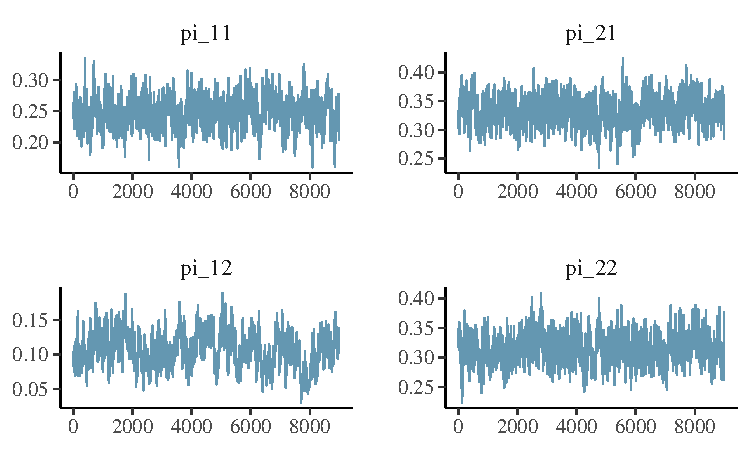
\includegraphics{dppaper_files/figure-latex/trace-plot-1} 

}

\caption{trace plots.}\label{fig:trace-plot}
\end{figure}

To see if there is evidence of gender bias we can look at the odds ratio.
Specifically, we look at the odds of a male being admitted to
that of female. A higher odds ratio would indicate a bias
favoring males. Figure \ref{fig:post-or-density} shows the posterior draws
from the dapper model. The large odds ratio values would seem
to indicate there is bias favoring the males. See (Bickel, Hammel, and O'Connell 1975) for
an explanation of the ``paradox'' of this result.

\begin{figure}

{\centering 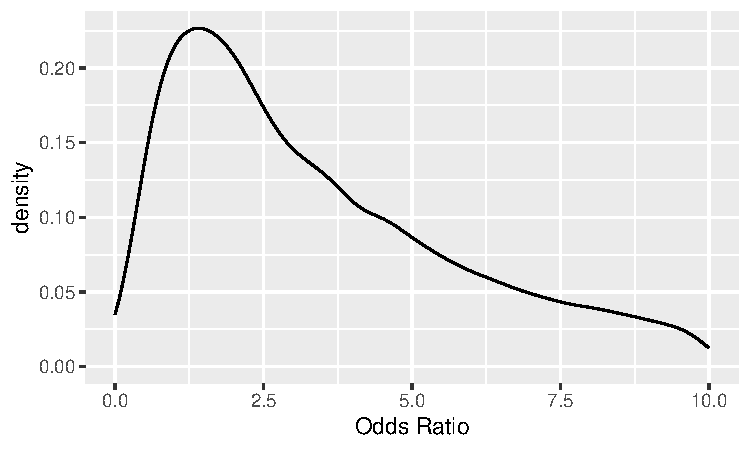
\includegraphics{dppaper_files/figure-latex/post-or-density-1} 

}

\caption{posterior density estimate for the odds ratio using 9000 MCMC draws.}\label{fig:post-or-density}
\end{figure}

For comparison, we run a standard Bayesian analysis on the
noise infused table ignoring the privacy mechanism. This will
correspond exactly to the model defined in the \texttt{post\_f} component.
Figure \ref{fig:post-or-compare} shows a density estimate for the odds ratio
under the confidential and noisy data. The posterior
distribution for the odds ratio under the noisy data
is shifted significantly, indicating a large degree of bias.
Looking at left hand plot in figure \ref{fig:post-or-compare} shows the MAP estimate from \texttt{dapper}
is similar to that in the case of the confidential data.
The width of the posterior is also much larger since
it properly accounts for the uncertainty due to the privacy mechanism. This
illustrates the dangers of ignoring the privacy mechanism. The naive
analysis not only has bias, but also severely underestimate the
uncertainty associated with the odds ratio estimate.

\begin{figure}

{\centering 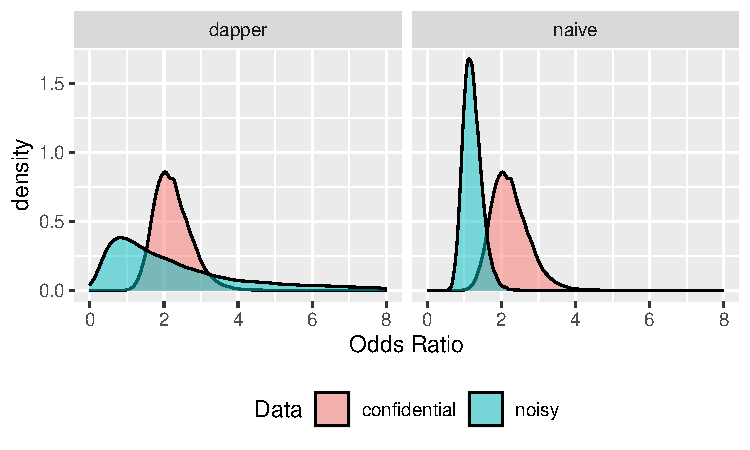
\includegraphics{dppaper_files/figure-latex/post-or-compare-1} 

}

\caption{comparison.}\label{fig:post-or-compare}
\end{figure}

\hypertarget{linear-regression}{%
\subsection{Linear Regression}\label{linear-regression}}

Below we review an application of \texttt{dapper} to an example
presented in (Ju et al. 2022) where they apply a Laplace privacy
mechanism to a sufficient summary statistic for a linear regression model.
Let \(\{(x_i,y_i)\}_{i=1}^{n}\) be the original, confidential data with \(x_i \in \mathbb{R}^2\).
They assume the true data generating process follows the model

\[
\begin{aligned}
y &= -1.79 -2.89x_1 -0.66x_2 + \epsilon\\
\epsilon &\sim N(0,2^2)\\
\binom{x_1}{x_2} &\sim N_{2}(\mu, I_2)\\
\mu &= \binom{0.9}{-1.17}.
\end{aligned}
\]

Note, in most settings involving linear regression, the covariates are assumed to be
fixed, known constants. Thus the formulation above is a departure from the norm since
we are assuming a random design matrix. More details on why this framing is necessary
will be provided later when describing the latent model.

The paper considers the scenario where one desires to publicly release the
sufficient summary statistics

\[
s(x,y) = (x^Ty, y^Ty, x^Tx).
\]

This summary statistic satisfies the additive record property since \(s(x,y) = \sum_{i=1}^{n} t(x_i, y_i)\)
where

\[
t(x_i,y_i) = ((x_{i})^T y_i, y_i^2, (x_{i})^T x_i),
\]

with \(\epsilon\)-DP privacy guarantees. To achieve this guarantee it is
necessary to bound the value of the statistic. This will ensure
a data point cannot be too ``unique.'' Intuitively, an outlier is
easy to identify, so in essence we want to make sure no data point
is an extreme outlier. In the language of differential
privacy, this equates to bounding the global sensitivity. This was accomplished
by clamping the data. More precisely, we define
the clamp function \([z] := \min\{\max\{z,-10\}, 10\}\) which truncates a value
\(z\) so that it falls into the interval \([-10,10]\). Furthermore, we let \(\tilde{z} := [z]/10\)
denote the normalized clamped value of \(z\). The clamped statistic is

\[
t(x_i,y_i) = ((\tilde{x}^{i})^T \tilde{y}_i, \tilde{y}_i^2, (\tilde{x}_{i})^T \tilde{x}_i).
\]

Ignoring duplicate entries, the global sensitivity is \(\Delta = p^2 + 3p + 3\) (wrong calculation, FIX!).
Using the Laplace mechanism, \(\epsilon\)-DP privacy can thus be achieved by adding i.i.d. Laplace\((0, \Delta/\epsilon)\)
error to each unique entry.

\begin{enumerate}
\def\labelenumi{\arabic{enumi}.}
\item
  \texttt{latent\_f}: Since the privacy mechanism involves injecting noise into the design
  matrix, it is not possible to use the standard approach where one assumes the design
  matrix is a fixed, known constant. Hence to draw a sample from the latent data generating
  process we use the relation \(f(x,y) = f(x)f(y \mid x)\). In this formulation,
  it is necessary to specify a distribution on the covariates \(x\).

\begin{verbatim}
latent_f <- function(theta) {
  xmat <- MASS::mvrnorm(50 , mu = c(.9,-1.17), Sigma = diag(2))
  y <- cbind(1,xmat) %*% theta + rnorm(1, sd = sqrt(2))
  cbind(y,xmat)
}
\end{verbatim}
\item
  \texttt{post\_f}: Given confidential data \(X\) we can derive the posterior analytically
  using a normal prior on \(\beta\).
  \[
  \begin{aligned}
  \beta &\sim N_{p+1}(0, \tau^2 I_{p+1})\\
  \beta \mid x,y &\sim N(\mu_n, \Sigma_n)\\
  \Sigma_n &= (x^Tx/\sigma^2 + I_{p+1}/\tau^2)^{-1}\\
  \mu_n &= \Sigma_n(x^Ty)/\sigma^2
  \end{aligned}
  \]
  In the example, we use \(\sigma^2 = 2\) and \(\tau^2 = 4\).

\begin{verbatim}
post_f <- function(dmat, theta) {
  x <- cbind(1,dmat[,-1])
  y <- dmat[,1]

  ps_s2 <- solve((1/2) * t(x) %*% x + (1/4) * diag(3))
  ps_m <- ps_s2 %*% (t(x) %*% y) * (1/2)

  MASS::mvrnorm(1, mu = ps_m, Sigma = ps_s2)
}
\end{verbatim}
\item
  \texttt{st\_f}: The summary statistic contains duplicate
  entries. We can considerable reduce the dimension of the
  statistic by only considering unique entries. The \texttt{clamp\_data}
  function is used to bound the statistic to give a finite
  global sensitivity.

\begin{verbatim}
clamp_data <- function(dmat) {
  pmin(pmax(dmat,-10),10) / 10
}

st_f <- function(dmat) {
  sdp_mat <- clamp_data(dmat)
  ydp <- sdp_mat[,1, drop = FALSE]
  xdp <- cbind(1,sdp_mat[,-1, drop = FALSE])

  s1 <- t(xdp) %*% ydp
  s2 <- t(ydp) %*% ydp
  s3 <- t(xdp) %*% xdp

  ur_s1 <- c(s1)
  ur_s2 <- c(s2)
  ur_s3 <- s3[upper.tri(s3,diag = TRUE)][-1]
  c(ur_s1,ur_s2,ur_s3)
}
\end{verbatim}
\item
  \texttt{priv\_f}: Privacy Mechanism
  adds Laplace\((0, \Delta/\epsilon)\) error to each unique entry
  of the statistic. In this example, \(\Delta = 13\) and \(\epsilon = 10\).

\begin{verbatim}
#deltaa <- 13
#epsilon <- 10
priv_f <- function(sdp, zt) {
  sum(VGAM::dlaplace(sdp - zt, 0, 13/10, log = TRUE))
}
\end{verbatim}
\end{enumerate}

First we simulate fake data using the aforementioned privacy mechanism.
In the example, we use \(n = 50\) observations.

\begin{verbatim}
deltaa <- 13
epsilon <- 10
n <- 50

xmat <- MASS::mvrnorm(n, mu = c(.9,-1.17), Sigma = diag(2))
beta <- c(-1.79, -2.89, -0.66)
y <- cbind(1,xmat) %*% beta + rnorm(n, sd = sqrt(2))

#clamp the confidential data in xmat
sdp <- st_f(cbind(y,xmat))

#add Laplace noise 
sdp <- sdp + VGAM::rlaplace(length(sdp), location = 0, scale = deltaa/epsilon)
\end{verbatim}

We construct a privacy model using the \texttt{new\_privacy} function and
make 25,000 MCMC draws with a burn in of 1000 draws.

\begin{verbatim}
library(progressr)

dmod <- new_privacy(post_f   = post_f,
                    latent_f = latent_f,
                    priv_f   = priv_f,
                    st_f     = st_f,
                    npar     = 3,
                    varnames = c("beta0", "beta1", "beta2"))


with_progress({
dp_out <- dapper_sample(dmod,
                        sdp = sdp,
                        niter = 25000,
                        warmup = 1000,
                        chains = 1,
                        init_par = rep(0,3))
})
\end{verbatim}

For comparison, we consider a Bayesian analysis where the design matrix
is a fixed known constant and \(\sigma^2\) is known. Using the
diffuse prior \(f(\beta) \propto 1\) leads to normal posterior.
\[
\begin{aligned}
f(\beta \mid x,y, \sigma^2) &\sim N(\hat{\beta}, \hat{\Sigma})\\
\hat{\mu} &= (x^Tx)^{-1}xy\\
\hat{\Sigma} &= \sigma^{2}(x^Tx)^{-1}
\end{aligned}
\]

The posterior can be written as a function of \(s(x,y)\). Since
we only have access to the noisy version \(s_{dp}\) we can
attempt to reconstruct the posterior be extracting the
relevant entries which is done below.

\begin{verbatim}
#x^Ty
s1 <- sdp[1:3]

#y^Ty
s2 <- sdp[4]

#x^Tx
s3 <- matrix(0, nrow = 3, ncol = 3)
s3[upper.tri(s3, diag = TRUE)] <- c(100, sdp[5:9])
s3[lower.tri(s3)] <- s3[upper.tri(s3)]
\end{verbatim}

Because of the injected privacy noise, the reconstructed
\((x^Tx)^{-1}\) matrix is not positive definite. As
a naive solution we use the algorithm proposed\\
in (Higham 1988) to find the closest positive semi-definite matrix
as determined by the Forbenius norm. The \texttt{pracma}
package contains an implementation via the \texttt{nearest\_psd}
function.

\begin{verbatim}
s3 <- pracma::nearest_spd(solve(s3))
bhat <- s3 %*% s1
sigma_hat <- 2 * s3
\end{verbatim}

Figure \ref{fig:regression-compare} shows the posterior density estimates for the \(\beta\) coefficients.

\begin{figure}

{\centering 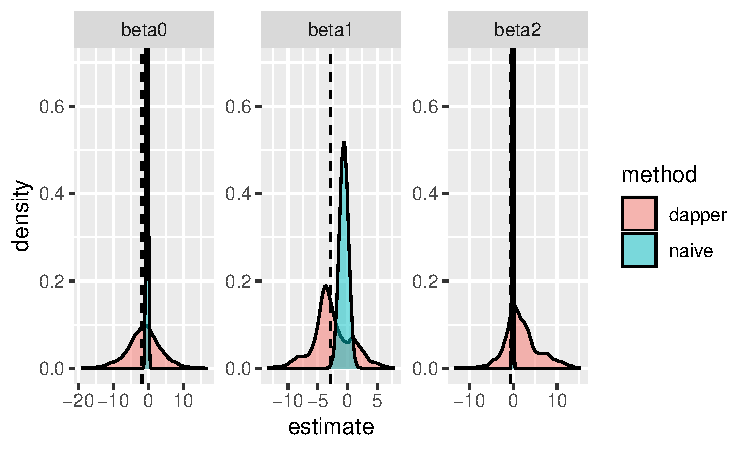
\includegraphics{dppaper_files/figure-latex/regression-compare-1} 

}

\caption{Comparison between dapper and a naive approach that ignores the privacy mechanism}\label{fig:regression-compare}
\end{figure}

\hypertarget{discussion}{%
\section{Discussion}\label{discussion}}

\hypertarget{poor-mixing}{%
\subsection{Poor Mixing}\label{poor-mixing}}

Mixing can be poor when the posterior under a given privacy mechanism is
much wider than the posterior that would arise using the confidential data. In
other words, when the privacy budget is small, poor mixing can be expected. The
rest of this section explores a toy example that will provide insight into this
phenomenon.

Suppose the confidential data consist of a single observation \(x \in \mathbb{R}\),
and consider the scenario where a user makes a request to view \(x\) and
in return receives \(s := x + \eta\), which is a noise infused version of \(x\).
For simplicity, we do not worry about constructing an \(\epsilon\)-DP privacy mechanism,
and take \(\eta \sim N(0, \epsilon^{-2})\) for some \(\epsilon > 0\). However, it
will still be useful to think of \(\epsilon\) as the privacy budget since smaller values
of \(\epsilon\) correspond to a larger amounts of noise. Using
a flat prior and a normally distributed likelihood results in
a normally distributed posterior described below.

\[
\begin{aligned}
f(\theta) &\propto 1\\
s \mid x &\sim N(x, \epsilon^{-2})\\
x \mid \theta &\sim N(\theta, \sigma^2)\\
\end{aligned}
\]

With the above model, the data augmentation process consist of the
two steps

\begin{itemize}
\item
  Step 1: Sample from \(x \mid \theta, s \sim N(\mu, \tau^2)\).
  \[
  \begin{aligned}
  \mu &= \dfrac{\dfrac{1}{\epsilon^{-2}}s + \dfrac{1}{\sigma^2}\theta}{\dfrac{1}{\epsilon^{-2}} + \dfrac{1}{\sigma^2}}\\
  \tau^2 &= \dfrac{1}{\dfrac{1}{\epsilon^{-2}} + \dfrac{1}{\sigma^2}}
  \end{aligned}
  \]
\item
  Step 2: Sample from \(\theta \mid x, s \sim N(x, \sigma^2)\).
\end{itemize}

It turns out the lag-1 auto-correlation is closely related
to the convergence rate of the chain in this example. (Liu and Wu 1999) showed
the lag-1 autocorrelation is related to the Bayesian fraction of missing information
and the latter, in fact, gives the exact convergence rate. The Bayesian fraction of missing information, \(\gamma\) is
defined as
\begin{align*}
\gamma &:= 1 - \dfrac{E[Var(\theta \mid s, x) \mid s]}{Var(\theta \mid s)} = 1 - \dfrac{E[Var(\theta \mid x)]}{Var(\theta \mid s)}.
\end{align*}

plugging in the appropriate quantities gives us

\begin{align*}
\gamma &= 1 - \dfrac{\sigma^2}{\sigma^2 + \epsilon^{-2}} = 1 - \dfrac{1}{1 + \dfrac{\epsilon^{-2}}{\sigma^2}}.
\end{align*}

The chain converges faster as \(\gamma \to 0\) an slower as \(\gamma \to 1\).
From the right hand term in the above panel, we can see \(\gamma\)
depends only on \(\epsilon^{-2}/\sigma^2\) and as the privacy budget decreases (i.e.~more noise is being added to \(x\)),
\(\gamma \to 1\).

Thus when poor mixing is observed, we recommend seeing if increasing the privacy
budget helps. Unfortunately, if one is not at liberty to alter the privacy budget,
there is no quick fix. In the case where a small privacy budget results
in a posterior much more diffuse than under the confidential data set, one
can draw samples using the pseudo-likelihood scheme as proposed in (Andrieu and Roberts 2009). This
scheme fits in the same data augmentation framework as \texttt{dapper} but is not implemented.

\hypertarget{related-work}{%
\subsection{Related Work}\label{related-work}}

Adjusting statistical workflows to account for added noise in covariates
is extensively studied in the context of measurement error (e.g.~noisy sensor readings)
and there exists readily available tools for making the proper adjustments.
For textbook length treatments on the topic see (Yi 2017; Carroll et al. 2006).
Work in this area mostly focuses on methods which do not require fully specifying the
measurement error model, since this is often assumed unknown.
However, in differential privacy, the measurement error model is exactly known.
This difference, makes feasible some ideas which the measurement
error community has not previously considered (Smith 2011; Karwa, Kifer, and Slavković 2015b).

\hypertarget{summary}{%
\section{Summary}\label{summary}}

Currently, there is a dearth of software tools privacy researchers can use
to evaluate the impact of privacy mechanisms on statistical analyses.
While there have been tremendous gains in the theoretical aspects of privacy,
the lack of software resources to deploy and work with new privacy techniques has
hampered their adoption. This gap in capability has been noted by several
large industry entities who have begun building software ecosystems for
working with differential privacy. SmartNoise by Microsoft {[}insert citation{]}, for example,
is a tool for generating synthetic data that has differentially private guarantees.
However, the majority of these software tools only address privacy and not the
ensuing analysis, or if it does address the analysis, only for specific models.
Privacy researchers currently lack good tools for evaluating the impact
of privacy mechanisms on a statistical analysis.

Thus DAPPER helps fill an urgent need by providing researchers a way to evaluate
how a particular privacy mechanism might effect a statistical analysis. A notable
feature is its flexibility which allows the users to specify a custom
privacy mechanism. The benefit being that DAPPER can evaluate already
established privacy mechanisms and those that have yet to be discovered.

While DAPPER can be a nice addition to a privacy researcher's tool kit, there
is still considerably more work that can be done. From a methodological standpoint,
DAPPER suffers from slow convergence when the privacy budget is small which is problematic
because this is the scenario where a privacy mechanism can have the greatest impact
on a statistical analysis. On the computational end, without a statistic that satisfies
record additivity, computation time can be unpalatable.

\hypertarget{references}{%
\section*{References}\label{references}}
\addcontentsline{toc}{section}{References}

\hypertarget{refs}{}
\begin{CSLReferences}{1}{0}
\leavevmode\vadjust pre{\hypertarget{ref-Abowd2018}{}}%
Abowd, John M. 2018. {``The u.s. Census Bureau Adopts Differential Privacy.''} In \emph{Proceedings of the 24th ACM SIGKDD International Conference on Knowledge Discovery \&Amp; Data Mining}. KDD '18. ACM. \url{https://doi.org/10.1145/3219819.3226070}.

\leavevmode\vadjust pre{\hypertarget{ref-Andrieu2009}{}}%
Andrieu, Christophe, and Gareth O. Roberts. 2009. {``The Pseudo-Marginal Approach for Efficient Monte Carlo Computations.''} \emph{The Annals of Statistics} 37 (2). \url{https://doi.org/10.1214/07-aos574}.

\leavevmode\vadjust pre{\hypertarget{ref-Bickel1975}{}}%
Bickel, P. J., E. A. Hammel, and J. W. O'Connell. 1975. {``Sex Bias in Graduate Admissions: Data from Berkeley: Measuring Bias Is Harder Than Is Usually Assumed, and the Evidence Is Sometimes Contrary to Expectation.''} \emph{Science} 187 (4175): 398--404. \url{https://doi.org/10.1126/science.187.4175.398}.

\leavevmode\vadjust pre{\hypertarget{ref-TopDown}{}}%
Bureau, U. S. Census. 2023. {``Disclosure Avoidance and the 2020 Census: How the TopDown Algorithm Works.''} 2023. \url{https://www.census.gov/library/publications/2023/decennial/c2020br-04.html}.

\leavevmode\vadjust pre{\hypertarget{ref-Carroll2006}{}}%
Carroll, Raymond J., David Ruppert, Leonard A. Stefanski, and Ciprian M. Crainiceanu. 2006. \emph{Measurement Error in Nonlinear Models}. Chapman; Hall/CRC. \url{https://doi.org/10.1201/9781420010138}.

\leavevmode\vadjust pre{\hypertarget{ref-ding2017collecting}{}}%
Ding, Bolin, Janardhan Kulkarni, and Sergey Yekhanin. 2017. {``Collecting Telemetry Data Privately.''} \url{https://arxiv.org/abs/1712.01524}.

\leavevmode\vadjust pre{\hypertarget{ref-Dwork2006}{}}%
Dwork, Cynthia, Frank McSherry, Kobbi Nissim, and Adam Smith. 2006. {``Calibrating Noise to Sensitivity in Private Data Analysis.''} In \emph{Lecture Notes in Computer Science}, 265--84. Springer Berlin Heidelberg. \url{https://doi.org/10.1007/11681878_14}.

\leavevmode\vadjust pre{\hypertarget{ref-Erlingsson_2014}{}}%
Erlingsson, Úlfar, Vasyl Pihur, and Aleksandra Korolova. 2014. {``RAPPOR: Randomized Aggregatable Privacy-Preserving Ordinal Response.''} In \emph{Proceedings of the 2014 ACM SIGSAC Conference on Computer and Communications Security}. CCS'14. ACM. \url{https://doi.org/10.1145/2660267.2660348}.

\leavevmode\vadjust pre{\hypertarget{ref-Gong2022}{}}%
Gong, Ruobin. 2022. {``Transparent Privacy Is Principled Privacy.''} \emph{Harvard Data Science Review}, no. Special Issue 2 (June). \url{https://doi.org/10.1162/99608f92.b5d3faaa}.

\leavevmode\vadjust pre{\hypertarget{ref-Higham1988}{}}%
Higham, Nicholas J. 1988. {``Computing a Nearest Symmetric Positive Semidefinite Matrix.''} \emph{Linear Algebra and Its Applications} 103 (May): 103--18. \url{https://doi.org/10.1016/0024-3795(88)90223-6}.

\leavevmode\vadjust pre{\hypertarget{ref-Hotz2022}{}}%
Hotz, V. Joseph, Christopher R. Bollinger, Tatiana Komarova, Charles F. Manski, Robert A. Moffitt, Denis Nekipelov, Aaron Sojourner, and Bruce D. Spencer. 2022. {``Balancing Data Privacy and Usability in the Federal Statistical System.''} \emph{Proceedings of the National Academy of Sciences} 119 (31). \url{https://doi.org/10.1073/pnas.2104906119}.

\leavevmode\vadjust pre{\hypertarget{ref-Ji2014}{}}%
Ji, Zhanglong, Zachary C. Lipton, and Charles Elkan. 2014. {``Differential Privacy and Machine Learning: A Survey and Review.''} \url{https://arxiv.org/abs/1412.7584}.

\leavevmode\vadjust pre{\hypertarget{ref-Ju2022}{}}%
Ju, Nianqiao, Jordan Awan, Ruobin Gong, and Vinayak Rao. 2022. {``Data Augmentation {MCMC} for Bayesian Inference from Privatized Data.''} In \emph{Advances in Neural Information Processing Systems}, edited by Alice H. Oh, Alekh Agarwal, Danielle Belgrave, and Kyunghyun Cho. \url{https://openreview.net/forum?id=tTWCQrgjuM}.

\leavevmode\vadjust pre{\hypertarget{ref-Karwa2015}{}}%
Karwa, Vishesh, Dan Kifer, and Aleksandra B. Slavković. 2015b. {``Private Posterior Distributions from Variational Approximations.''} \url{https://arxiv.org/abs/1511.07896}.

\leavevmode\vadjust pre{\hypertarget{ref-karwa2015private}{}}%
---------. 2015a. {``Private Posterior Distributions from Variational Approximations.''} \url{https://arxiv.org/abs/1511.07896}.

\leavevmode\vadjust pre{\hypertarget{ref-Kenny2021}{}}%
Kenny, Christopher T., Shiro Kuriwaki, Cory McCartan, Evan T. R. Rosenman, Tyler Simko, and Kosuke Imai. 2021. {``The Use of Differential Privacy for Census Data and Its Impact on Redistricting: The Case of the 2020 u.s. Census.''} \emph{Science Advances} 7 (41). \url{https://doi.org/10.1126/sciadv.abk3283}.

\leavevmode\vadjust pre{\hypertarget{ref-Liu1999}{}}%
Liu, Jun S., and Ying Nian Wu. 1999. {``Parameter Expansion for Data Augmentation.''} \emph{Journal of the American Statistical Association} 94 (448): 1264--74. \url{https://doi.org/10.1080/01621459.1999.10473879}.

\leavevmode\vadjust pre{\hypertarget{ref-Robert2004}{}}%
Robert, Christian P., and George Casella. 2004. \emph{Monte Carlo Statistical Methods}. \emph{Springer Texts in Statistics}. Springer New York. \url{https://doi.org/10.1007/978-1-4757-4145-2}.

\leavevmode\vadjust pre{\hypertarget{ref-SantosLozada2020}{}}%
Santos-Lozada, Alexis R., Jeffrey T. Howard, and Ashton M. Verdery. 2020. {``How Differential Privacy Will Affect Our Understanding of Health Disparities in the United States.''} \emph{Proceedings of the National Academy of Sciences} 117 (24): 13405--12. \url{https://doi.org/10.1073/pnas.2003714117}.

\leavevmode\vadjust pre{\hypertarget{ref-Smith2011}{}}%
Smith, Adam. 2011. {``Privacy-Preserving Statistical Estimation with Optimal Convergence Rates.''} In \emph{Proceedings of the Forty-Third Annual ACM Symposium on Theory of Computing}. STOC'11. ACM. \url{https://doi.org/10.1145/1993636.1993743}.

\leavevmode\vadjust pre{\hypertarget{ref-tang2017privacy}{}}%
Tang, Jun, Aleksandra Korolova, Xiaolong Bai, Xueqiang Wang, and Xiaofeng Wang. 2017. {``Privacy Loss in Apple's Implementation of Differential Privacy on MacOS 10.12.''} \url{https://arxiv.org/abs/1709.02753}.

\leavevmode\vadjust pre{\hypertarget{ref-Wang2018}{}}%
Wang, Yue, Daniel Kifer, Jaewoo Lee, and Vishesh Karwa. 2018. {``Statistical Approximating Distributions Under Differential Privacy.''} \emph{Journal of Privacy and Confidentiality} 8 (1). \url{https://doi.org/10.29012/jpc.666}.

\leavevmode\vadjust pre{\hypertarget{ref-NIPS2010_sherry}{}}%
Williams, Oliver, and Frank Mcsherry. 2010. {``Probabilistic Inference and Differential Privacy.''} In \emph{Advances in Neural Information Processing Systems}, edited by J. Lafferty, C. Williams, J. Shawe-Taylor, R. Zemel, and A. Culotta. Vol. 23. Curran Associates, Inc. \url{https://proceedings.neurips.cc/paper_files/paper/2010/file/fb60d411a5c5b72b2e7d3527cfc84fd0-Paper.pdf}.

\leavevmode\vadjust pre{\hypertarget{ref-Winkler2021}{}}%
Winkler, Richelle L., Jaclyn L. Butler, Katherine J. Curtis, and David Egan-Robertson. 2021. {``Differential Privacy and the Accuracy of County-Level Net Migration Estimates.''} \emph{Population Research and Policy Review} 41 (2): 417--35. \url{https://doi.org/10.1007/s11113-021-09664-5}.

\leavevmode\vadjust pre{\hypertarget{ref-Yi2017}{}}%
Yi, Grace Y. 2017. \emph{Statistical Analysis with Measurement Error or Misclassification}. \emph{Springer Series in Statistics}. Springer New York. \url{https://doi.org/10.1007/978-1-4939-6640-0}.

\end{CSLReferences}

\bibliography{RJreferences.bib}

\address{%
Kevin Eng\\
Rutgers University\\%
Department of Statistics\\ Piscataway, NJ 08854\\
%
\url{https://www.britannica.com/animal/quokka}\\%
%
\href{mailto:ke157@stat.rutgers.edu}{\nolinkurl{ke157@stat.rutgers.edu}}%
}

\address{%
Jordan A. Awan\\
Purdue University\\%
Department of Statistics\\ West Lafayette, IN 47907\\
%
\url{https://www.britannica.com/animal/quokka}\\%
%
\href{mailto:jawan@purdue.edu}{\nolinkurl{jawan@purdue.edu}}%
}

\address{%
Ruobin Gong\\
Rutgers University\\%
Department of Statistics\\ Piscataway, NJ 08854\\
%
\url{https://www.britannica.com/animal/quokka}\\%
%
\href{mailto:ruobin.gong@rutgers.edu}{\nolinkurl{ruobin.gong@rutgers.edu}}%
}

\address{%
Nianqiao Phyllis Ju\\
Purdue University\\%
Department of Statistics\\ West Lafayette, IN 47907\\
%
\url{https://www.britannica.com/animal/quokka}\\%
%
\href{mailto:nianqiao@purdue.edu}{\nolinkurl{nianqiao@purdue.edu}}%
}

\address{%
Vinayak A. Rao\\
Purdue University\\%
Department of Statistics\\ West Lafayette, IN 47907\\
%
\url{https://www.britannica.com/animal/quokka}\\%
%
\href{mailto:varao@purdue.edu}{\nolinkurl{varao@purdue.edu}}%
}
